\chapter{FCHC}

In two dimensions, we are lucky to find hexagon -- a symmetric polygon that covers whole 2D plane and possesses sufficient rotational symmetry to make a good lattice for FHP.

In three dimensions, we have five symmetric candidates for LGCA, so--called Plato solids, but none of them works.
Dodecahedron and icosahedron might have sufficient rotational symmetry (interestingly, they share the group of symmetries)
but they do not cover whole 3D space uniformly. Only the cube does but LGCA build on a rectangular lattice would suffer from the same diseases as HPP -- insufficient rotational symmetry and insufficient degrees of freedom in the nodes.

Short analysis \cite{wolf} shows that in 5 and more dimensions, we have only three symmetric solids -- simplex, hypercube and its dual solid. None of them fits.

\bigskip

Fortunately, in four dimensions, we have three extra symmetric solids and one of them actually works.

\section{Face-centered hypercube}
Face-centered hypercube (we will use the shortcut FCHC) is the suitable solid for LGCA in four dimensions. It can be defined by its 24 vertices with the Cartesian coordinates

\begin{tabular}{cccc}
\\
($\pm 1$,& $\pm 1$,& $0$,& $0$),\\
($\pm 1$,& $0$,& $\pm 1$,& $0$),\\
($\pm 1$,& $0$,& $0$,& $\pm 1$),\\
($0$,& $\pm 1$,& $\pm 1$,& $0$),\\
($0$,& $\pm 1$,& $0$,& $\pm 1$),\\
($0$,& $0$,& $\pm 1$,& $\pm 1$).\\
\\
\end{tabular}

These 24 vertices correspond to 24 lattice vectors in four dimensions but if we project them into three dimensions (by deleting the fourth coordinate $q_4$) we get only 18 lattice vectors

\begin{tabular}{cccc}
\\
($\pm 1$,& $\pm 1$,& $0$),\\
($\pm 1$,& $0$,& $\pm 1$),\\
($\pm 1$,& $0$,& $0$),\\
( $0$,& $\pm 1$,& $\pm 1$),\\
( $0$,& $\pm 1$,& $0$),\\
( $0$,& $0$,& $\pm 1$).\\
\\
\end{tabular}

\begin{figure}
 \centering
 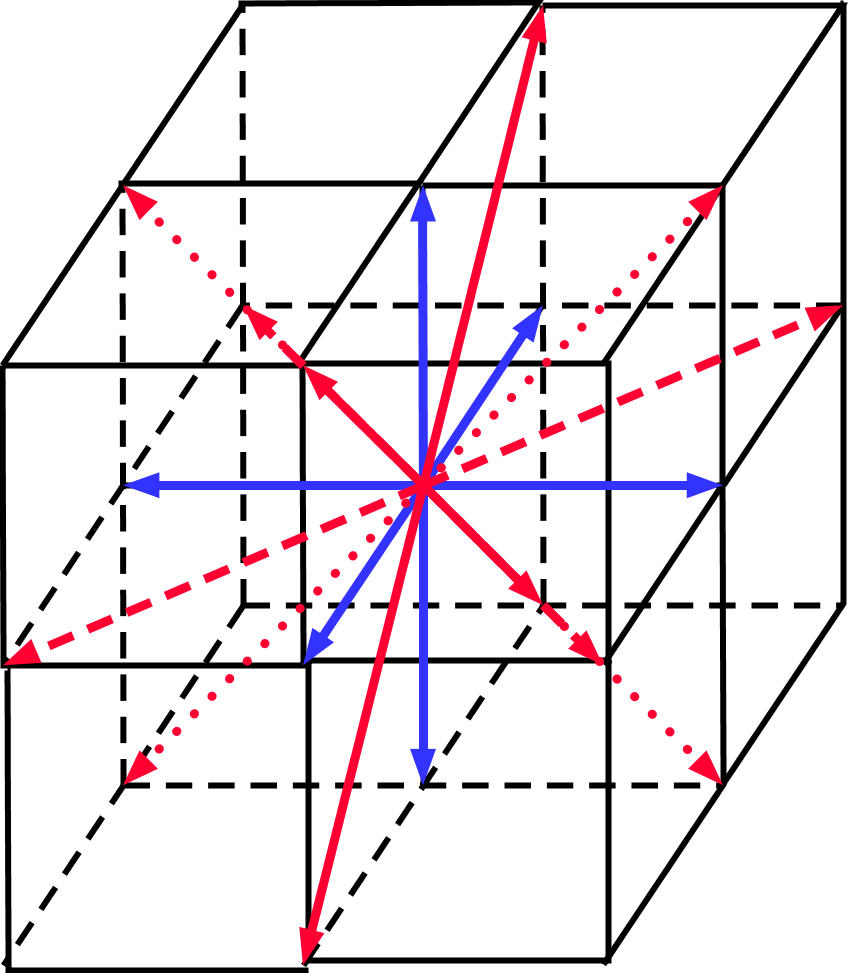
\includegraphics[width=0.6\textwidth]{../obrazky/FCHC}
 \label{fchc}
 \caption{Projection of the lattice vectors into 3D. Red arrows are projections of vectors with $q_4 = 0$,
 blue arrows with $q_4 = \pm 1$.}
\end{figure}

For $q_4 = 0$ we have 12 lattice vectors (red lines on the figure \ref{fchc}), each vector corresponds to the single cell only, so at most one particle propagates along each.
%Hence, at most one particle propagates along each of these vectors.

For both $q_4 = -1$ and $q_4 = 1$ we obtain same six lattice vectors (blue lines on the figure \ref{fchc}). Each vector corresponds to the two cells, hence two particles can propagate along each vector.

In the end, the $3D$ projection of the FCHC lattice leads to the rectangular grid, so the position of the nodes can be denoted by 3 Cartesian integer coordinates.
Each node is connected to 18 neighbors by the lattice vectors of Fig.\ \ref{fchc}, and 24 particles can propagate along them in the single step.

\section{Collision rules for FCHC}

The FCHC lattice that we have just described was proposed already by Frisch et.\ al.\ in 1986.
However, they did not propose any recipe for a collision step. It is easy to understand why it is not a simple task.

There are 24 cells in each node, so the node can acquire $2^{24} = 16~777~216$ different states (that can be represented by 24 bits). It was easy to specify the collision rule for FHP in one simple table, but how do you specify rules for millions of states?

In the subsequent section we will show how Henon answered to this challenge in his famous article \cite{henon}.

\bigskip

\subsection{Necessary conditions}

Let us review what are the necessary conditions that collision rules must fulfill:

\begin{enumerate}
\item number of particles is preserved;
\item total momentum is preserved;
\item no other quantity is preserved;
\item exclusion principle -- no two particles occupy one cell in the new state;
\item collision rules are invariant with respect to rotations and reflections of the node;
\item collisions satisfy the semi-detailed balance.
\end{enumerate}

Henon proposed his own conditions on the collisions and showed that all conditions above are automatically fulfilled.

\begin{enumerate}
\item All collisions are isometries of FCHC -- such transformations that preserve set of 24 lattice vectors above. It can be shown that this condition actually defines FHP collision set. For FCHC, this condition guarantees that conditions will be simple and leads us to the simple collision algorithm.

\item The choice of isometry is restricted by the momentum conservation only.
There are 7009 possible values of momentum. But considering that collision rules are invariant under isometries of FCHC, and due to first restriction that collisions are isometries, we can consider 37 momenta only.

\item We want shear viscosity to be as low as possible, so that we can go to higher Reynolds numbers in our simulations. Suppressing the viscosity means is achieved by shortening the mean free path of the particles. In other words, we wish to change as many bits in the collision as possible. We will call such collisions "optimal isometries".

\item The isometry is randomly chosen among optimal isometries.

\end{enumerate}

Having discussed the role of the isometries, let us define them properly.

\section{Isometries of FCHC} 

By $G$ we denote the group of isometries that preserve all 24 lattice vectors (or equivalently all vertexes of FCHC). Any isometry can be represented by $4 \times 4$ matrix
\begin{align}
M = 
\begin{bmatrix}
a_{11} & ... & a_{14} \\
... & & ... \\
a_{41} & ... & a_{44}
\end{bmatrix}.
\end{align}
Although the group G is of order 1152, it can be generated by five elements only,
but it will be more comfortable to employ the generating set consisting of 12 elements to be described in the following section.

\subsection{Generating set}
Isometries $S_{\alpha},~\alpha=1,2,3,4,$ are reflections over(?) plane $x_{\alpha} = 0$.
For example, $S_{1}$ is represented by the matrix
\begin{align}
S_1 = 
\left[\begin{array}{rrrr}
-1 & 0 & 0 & 0 \\
 0 & 1 & 0 & 0 \\
 0 & 0 & 1 & 0 \\
 0 & 0 & 0 & 1
\end{array}\right]
\end{align} 
that flips the sign of the first momentum coordinate $q_{1}$.

\bigskip

Another six isometries $P_{\alpha \beta}$ are reflections over plane $x_{\alpha} = x_{\beta}$.
For example, $P_{12}$ can be represented by matrix
\begin{align}
P_{12} =
\begin{bmatrix}
0 & 1 & 0 & 0 \\
1 & 0 & 0 & 0 \\
0 & 0 & 1 & 0 \\
0 & 0 & 0 & 1
\end{bmatrix}.
\end{align}
that swaps the first and second coordinates of the momentum.

Another isometry $\Sigma_1$ is reflection over plane $x_1 + x_4 = x_2 + x_3$ represented by matrix
\begin{align}
\Sigma_1 = \frac{1}{2}
\left[\begin{array}{rrrr}
1 & 1 & 1 & -1 \\
1 & 1 & -1 & 1 \\
1 & -1 & 1 & 1 \\
-1 & 1 & 1 & 1
\end{array}\right].
\end{align}

The last generating isometry $\Sigma_2$ is reflection over plane $x_1 = x_2 + x_3 + x_4$.
In matrix representation it reads
\begin{align}
\Sigma_2 = \frac{1}{2}
\left[\begin{array}{rrrr}
1 & 1 & 1 & 1 \\
1 & 1 & -1 & -1 \\
1 & -1 & 1 & -1 \\
1 & -1 & -1 & 1
\end{array}\right]
\end{align}

Any isometry of FCHC can be composed from these 12 isometries,
so it can be uniquely expressed by
\begin{align}
M = 
\begin{pmatrix}
I\\
S_4
\end{pmatrix}
\begin{pmatrix}
I\\
S_3
\end{pmatrix}
\begin{pmatrix}
I\\
S_2
\end{pmatrix}
\begin{pmatrix}
I\\
S_1
\end{pmatrix}
\begin{pmatrix}
I\\
P_{34}
\end{pmatrix}
\begin{pmatrix}
I\\
P_{23}\\
P_{24}
\end{pmatrix}
\begin{pmatrix}
I\\
P_{12}\\
P_{13}\\
P_{14}
\end{pmatrix}
\begin{pmatrix}
I\\
\Sigma_1\\
\Sigma_2
\end{pmatrix}
\end{align} 
where the brackets mean ``one of the isometries inside the bracket".


\subsection{Normalized momenta}
Normalized momenta are such momenta that their components fulfill the following two conditions:
\begin{enumerate}
\item $q_1 \geq q_2 \geq q_3 \geq q_4 \geq 0$,  \label{normMom}
\item $q_0 = 0$ or $q_1+g_4 = q_2 + q_3$.
\end{enumerate}


Henon specified collision rules for normalized momenta only. There is 37 normalized momenta (out of 7009 total) so he significantly simplified the job.

If the state has normalized momentum (i.e.\ fulfilling \ref{normMom}), we just look into table and pick any isometry that is offered for that momentum. However, if the state doesn't have normalized momentum,
\begin{enumerate}
\item we normalize it by applying an appropriate isometry on the state. Let us denote this isometry by $\Gamma$. In fact, this isometry is equivalent to the change of the coordinate system.

\item Now that we have state with normalized momenta, search in the table and pick an optimal isometry.

\item We go back to the previous coordinate system by applying isometry $\Gamma^{-1}$.
\end{enumerate}

\subsection{Optimal isometries}

However, in the step 2, we do not want to use all the isometries that conserve the momentum.
Optimally, we would like to change as many bits as possible (that minimizes mean free path of particles, and that leads to desired low viscosity).

Although no further reduction beyond 37 normalized momenta is possible,
some of these momenta share same optimal isometries, that lead to minimal viscosity and preserve momentum.

Based on that,  momenta can be divided into 12 classes, as we did in the table below.
First column specifies momentum, the second column specifies isometries that can be applied to this momentum. 
Before the simulations starts, we calculate optimal states for each of the $2^{24}$ initial states. Then, the collision step reduces to searching in this huge table and randomly choosing from the available states.

Back in the times when this algorithm was proposed and tested, the look-up table was considered too big, and several optimizations were proposed and implemented in CRAY-Asssebler \cite{wolf}. Despite that, the achieved update rate was lower then of the Pair-iteraction model, that we are presenting in the next chapter. 
%\begin{tabular}{ |p{1cm}||p{1cm}||p{0.5cm}|p{7cm}|  }
% \hline
% Class& $w_{min}$&\multicolumn{2}{|c|}{Optimal isometries} \\
% \hline
% \hline
% $1$	&	$1/2$	&	$1$	&	$P_{12}$\\
% $2$	&	$1/4$	&	$2$	&	$P_{23}P_{12},\,P_{23}P_{13}$\\
% $3$	&	$1/4$	&	$2$	&	$S_4\Sigma_1,\,S_4\Sigma_2$\\
% $4$	&	$1/2$	&	$1$	&	$S_4$\\
% $5$	&	$1/3$	&	$1$	&	$S_4P_{12}$\\
% $6$	&	$1/4$	&	$4$	&	$S_4\Sigma_1,\,S_4\Sigma_2,\,S_4P_{23}\Sigma_1,S_4P_{23}\Sigma_2$\\
% $7$	&	$1/3$	&	$1$	&	$S_4P_{23}$\\
% $8$	&	$1/4$	&	$4$	&	$P_{23}P_{12},\,P_{23}P_{13},\,S_4P_{23}P_{12},\,S_4P_{23}P_{12}$\\
% $9$	&	$1/3$	&	$3$	&	$S_4S_3,\,S_3P_{34},\,S_4P_{34}$\\
% $10$	&	$1/6$	&	$6$	&	$S_3P_{34}P_{12},\,S_4P_{34}P_{12},\,S_4S_3\Sigma_1,$\\
%		&			&			&	$S_4S_3P_{34}P_{12}\Sigma_1,\,S_4S_3\Sigma_2,\,P_{34}P_{12}\Sigma_2$\\
% $11$	&	$1/6$	&	$6$	&	$S_4S_2P_{23},\,S_4S_3P_{23},\,S_3S_2P_{24},$\\
% 		&			&			&	$S_4S_3P_{24},\,S_3S_2P_{34},\,S_4S_2P_{34}$\\
% $12$	&	$0$	&	$12$	&	$S_3S_1P_{34}P_{12},\,S_4S_1P_{34}P_{12},\,S_3S_2P_{34}P_{12},$\\
% 		&			&			&	$S_4S_2P_{34}P_{12},\,S_2S_1P_{24}P_{13},\,S_4S_1P_{13}P_{13},$\\
% 		&			&			&	$S_3S_2P_{24}P_{13},\,S_4S_3P_{24}P_{13},\,S_2S_1P_{23}P_{14},$\\
% 		&			&			&	$S_3S_1P_{23}P_{14},\,S_4S_2P_{23}P_{14},\,S_4S_3P_{23}P_{14}$\\ 
%\hline 
%\end{tabular}

%\begin{tabular}{ |p{1cm}||p{1cm}||p{0.5cm}|p{9cm}|  }
% \hline
% Class& $w_{min}$&\multicolumn{2}{|c|}{Optimal isometries} \\
% \hline
% \hline
% $1$	&	$1/2$	&	$1$	&	$P_{12}$\\
% $2$	&	$1/4$	&	$2$	&	$P_{23}P_{12},\,P_{23}P_{13}$\\
% $3$	&	$1/4$	&	$2$	&	$S_4\Sigma_1,\,S_4\Sigma_2$\\
% $4$	&	$1/2$	&	$1$	&	$S_4$\\
% $5$	&	$1/3$	&	$1$	&	$S_4P_{12}$\\
% $6$	&	$1/4$	&	$4$	&	$S_4\Sigma_1,\,S_4\Sigma_2,\,S_4P_{23}\Sigma_1,S_4P_{23}\Sigma_2$\\
% $7$	&	$1/3$	&	$1$	&	$S_4P_{23}$\\
% $8$	&	$1/4$	&	$4$	&	$P_{23}P_{12},\,P_{23}P_{13},\,S_4P_{23}P_{12},\,S_4P_{23}P_{12}$\\
% $9$	&	$1/3$	&	$3$	&	$S_4S_3,\,S_3P_{34},\,S_4P_{34}$\\
% $10$	&	$1/6$	&	$6$	&	$S_3P_{34}P_{12},\,S_4P_{34}P_{12},\,S_4S_3\Sigma_1,\,S_4S_3P_{34}P_{12}\Sigma_1,$\\
%		&			&			&	$S_4S_3\Sigma_2,\,P_{34}P_{12}\Sigma_2$\\
% $11$	&	$1/6$	&	$6$	&	$S_4S_2P_{23},\,S_4S_3P_{23},\,S_3S_2P_{24},\,S_4S_3P_{24},$\\
% 		&			&			&	$S_3S_2P_{34},\,S_4S_2P_{34}$\\
% $12$	&	$0$	&	$12$	&	$S_3S_1P_{34}P_{12},\,S_4S_1P_{34}P_{12},\,S_3S_2P_{34}P_{12},\,S_4S_2P_{34}P_{12},$\\
% 		&			&			&	$S_2S_1P_{24}P_{13},\,S_4S_1P_{13}P_{13},\,S_3S_2P_{24}P_{13},\,S_4S_3P_{24}P_{13},$\\
% 		&			&			&	$S_2S_1P_{23}P_{14},\,S_3S_1P_{23}P_{14},\,S_4S_2P_{23}P_{14},\,S_4S_3P_{23}P_{14}$\\ 
%\hline 
%\end{tabular}

\begin{tabular}{ |p{4cm}||p{8.9cm}|  }
 \hline
 Normalized momenta	&	Optimal isometries \\
 \hline
 \hline
 $q_1=q_2>q_3>q_4>0$	&	$P_{12}$\\
 \hline
 $q_1=q_2=q_3>q_4>0$	&	$P_{23}P_{12},\,P_{23}P_{13}$\\
 \hline
 $q_1>q_2>q_3>q_4=0,$	&	$S_4\Sigma_1,\,S_4\Sigma_2$\\
 $q_1=q_2+q_3$				&	\\
 \hline
 $q_1>q_2>q_3>q_4=0,$	&	$S_4$\\
 $q_1 \neq q_2+q_3$		&	\\
 \hline
 $q_1=q_2>q_3>q_4=0$	&	$S_4P_{12}$\\
 \hline
 $q_1>q_2=q_3>q_4=0$	&	$S_4\Sigma_1,\,S_4\Sigma_2,\,S_4P_{23}\Sigma_1,S_4P_{23}\Sigma_2$\\
 \hline
 $q_1>q_2=q_3>q_4=0,$	&	$S_4P_{23}$\\
 $q_q=2q_2$					&	\\
 \hline
 $q_1>q_2=q_3>q_4=0,$	&	$P_{23}P_{12},\,P_{23}P_{13},\,S_4P_{23}P_{12},\,S_4P_{23}P_{12}$\\
 $q_1 \neq 2q_2$				&	\\
 \hline
 $q_1=q_2=q_3>q_4=0$	&	$S_4S_3,\,S_3P_{34},\,S_4P_{34}$\\
 \hline
 $q_1>q_2=q_3=q_4=0$	&	$S_3P_{34}P_{12},\,S_4P_{34}P_{12},\,S_4S_3\Sigma_1,\,S_4S_3P_{34}P_{12}\Sigma_1,$\\
									&	$S_4S_3\Sigma_2,\,P_{34}P_{12}\Sigma_2$\\
 \hline
 $q_1>q_2=q_3=q_4=0$	&	$S_4S_2P_{23},\,S_4S_3P_{23},\,S_3S_2P_{24},\,S_4S_3P_{24},$\\
									&	$S_3S_2P_{34},\,S_4S_2P_{34}$\\
\hline
 $q_1=q_2=q_3=q_4=0$	&	$S_3S_1P_{34}P_{12},\,S_4S_1P_{34}P_{12},\,S_3S_2P_{34}P_{12},\,S_4S_2P_{34}P_{12},$\\
									&	$S_2S_1P_{24}P_{13},\,S_4S_1P_{13}P_{13},\,S_3S_2P_{24}P_{13},\,S_4S_3P_{24}P_{13},$\\
									&	$S_2S_1P_{23}P_{14},\,S_3S_1P_{23}P_{14},\,S_4S_2P_{23}P_{14},\,S_4S_3P_{23}P_{14}$\\ 
\hline 
\end{tabular}

%\begin{figure}
% \centering
% \includegraphics[width=1\textwidth]{./img/Optimal}
%% \label{optimalies}
% \caption{Optimal isometries for 12 momenta classes}
%\end{figure}